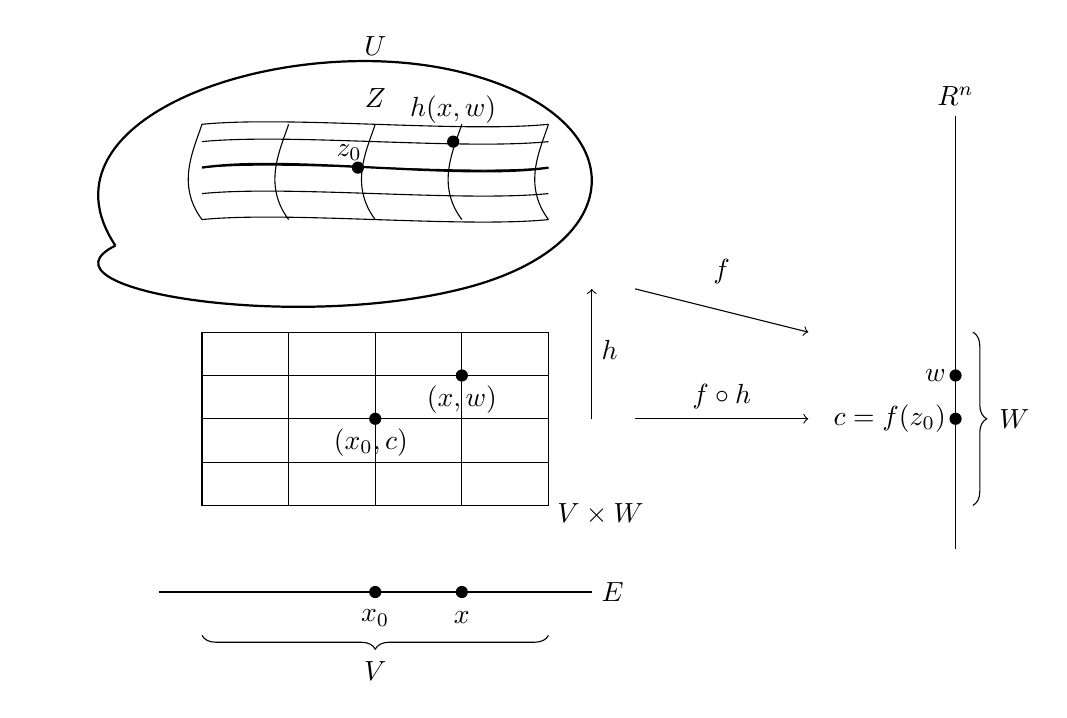
\begin{tikzpicture}[scale=1.1]

% ======================
% REGIÓN SUPERIOR (U)
% ======================

% Contorno tipo "orgánico"
\draw[thick] (-5,1.5) .. controls (-6,3) and (-3,4) .. (-1,3.5)
             .. controls (1,3) and (1,1.5) .. (-1,1)
             .. controls (-3,0.5) and (-6,1) .. (-5,1.5);

\node at (-2,3.8) {$U$};
\node at (-2,3.2) {$Z$};

% "Fibras" (curvas horizontales suaves)
\foreach \y in {1.8,2.1,2.4,2.7,2.9} {
    \draw (-4,\y)
    .. controls (-3,{\y+0.1}) and (-1,{\y-0.1}) ..
    (0,\y);
}

% Fibra destacada (la del punto a)
\draw[thick]
(-4,2.4)
.. controls (-3,2.55) and (-1,2.25) ..
(0,2.4);

% Líneas verticales (estructura tipo producto)
\draw (-3,1.8)
.. controls (-3.3,2.2) and (-3.1,2.6) ..
(-3,2.9);

\draw (-2,1.8)
.. controls (-2.3,2.2) and (-2.1,2.6) ..
(-2,2.9);

\draw (-1,1.8)
.. controls (-1.3,2.2) and (-1.1,2.6) ..
(-1,2.9);

\draw (-4,1.8)
.. controls (-4.3,2.2) and (-4.1,2.6) ..
(-4,2.9);

\draw (0,1.8)
.. controls (-0.3,2.2) and (-0.1,2.6) ..
(0,2.9);


% Punto a
\fill (-1.1,2.7) circle (2pt);
  \node[above] at (-1.1,2.8) {$h(x,w)$};

% Punto izquierda
\fill (-2.2,2.4) circle (2pt);
\node[above] at (-2.3,2.37) {$z_0$};

% ======================
% REGIÓN INFERIOR (V x W)
% ======================

\draw (-4,-1.5) rectangle (0,0.5);
\node at (0.6,-1.6) {$V\times W$};
% Grid
\foreach \x in {-4,-3,-2,-1,0} {
    \draw (\x,-1.5) -- (\x,0.5);
}
\foreach \y in {-1,-0.5,0} {
    \draw (-4,\y) -- (0,\y);
}

% Punto (a1,c)
\fill (-2,-0.5) circle (2pt);
  \node[below] at (-2.05,-0.5) {$(x_0,c)$};

% Punto (x,c)
\fill (-1,0) circle (2pt);
\node[below] at (-1,0) {$(x,w)$};

% Flecha h
\draw[->] (0.5,-0.5) -- (0.5,1);
\node[right] at (0.5,0.3) {$h$};

% ======================
% EJE INFERIOR (R^m)
% ======================

\draw (-4.5,-2.5) -- (0.5,-2.5);
\node[right] at (0.5,-2.5) {$E$};

\fill (-1,-2.5) circle (2pt);
\node at (-1,-2.8) {$x$};
\fill (-2,-2.5) circle (2pt);
\node at (-2,-2.8) {$x_0$};
% Segmento W
\draw[
  decorate,
  decoration={brace, mirror, amplitude=5pt}
]
(-4,-3) -- (0,-3)
node[midway, below=6pt] {$V$};

% ======================
% LADO DERECHO (R^n)
% ======================

\draw (4.7,-2) -- (4.7,3);
\node[above] at (4.7,3) {$\mathbb{R}^n$};

% Segmento W
\draw[
  decorate,
  decoration={brace, mirror, amplitude=5pt}
]
(4.9,-1.5) -- (4.9,0.5)
node[midway, right=6pt] {$W$};

\fill (4.7,-0.5) circle (2pt);
\node[left] at (4.7,-0.5) {$c=f(z_0)$};

\fill (4.7,0) circle (2pt);
\node[left] at (4.7,0) {$w$};

% Flecha f diagonal
\draw[->] (1,1) -- (3,0.5);
\node at (2,1.2) {$f$};

% Flecha horizontal
\draw[->] (1,-0.5) -- (3,-0.5);
\node[above] at (2,-0.5) {$f\circ h$};

\end{tikzpicture}
